\documentclass{article}
\usepackage{amssymb}
\usepackage{amsmath}
\usepackage{mathtools}
\usepackage{cancel}
\usepackage{tikz}
\usepackage{hyperref}
\usepackage{circuitikz}
\usepackage{float}
\usepackage{afterpage}
\usepackage{pgfplots}
\usepackage{textcomp}
\usepgfplotslibrary{groupplots}
\usetikzlibrary{calc, arrows}
\newtheorem{theorem}{Theorem}
\newtheorem{definition}{Definition}
\newtheorem{corollary}{Corollary}
\newtheorem{proof}{Proof}
\tikzstyle{int}=[draw, fill=blue!20, minimum size=2em]
\tikzstyle{init} = [pin edge={to-,thin,black}]

\tikzstyle{block} = [draw, fill=blue!20, rectangle, 
    minimum height=3em, minimum width=6em]
\tikzstyle{sum} = [draw, fill=blue!20, circle, node distance=1cm]
\tikzstyle{input} = [coordinate]
\tikzstyle{output} = [coordinate]
\tikzstyle{pinstyle} = [pin edge={to-,thin,black}]
\tikzstyle{filter} = [draw, fill=blue!20, rectangle, 
minimum height=3em, minimum width=6em, align=center, text width=2cm]

\DeclareMathOperator*{\argmin}{argmin}

\begin{document}
\title{EE123 Course Notes}
\author{Anmol Parande}
\date{Spring 2020 - Professor Miki Lustig}
\maketitle
\textbf{Disclaimer: }These notes reflect EE123 when I took the course (Spring 2020). They may not accurately reflect current course content, so use at your own risk.
If you find any typos, errors, etc, please raise an issue on the \href{https://github.com/parandea17/BerkeleyNotes}{GitHub repository}.\\
\tableofcontents
\newpage
\section{The DFT}
Whereas the CTFT takes a continuous signal and outputs a continuous frequency spectrum and the DTFT takes a discrete signal
and outputs a continuous, periodic frequecy spectrum, the Discrete Fourier Transform takes a discrete finite signal and outputs
a discrete frequency spectrum. This is useful for signal processing because we cannot store infinite signals in a computers memory.
\begin{definition}
    For a length $N$ finite sequence $\{x[n]\}^{n-1}_{0}$, the Discrete Fourier Transform of the signal
    is a length N finite sequence $\{X[k]\}^{n-1}_{0}$ where
    $$X[k] = \sum_{n=0}^{N-1}{x[n]e^{-j\frac{2\pi}{N}kn}}$$
\end{definition}
One way to interpret the DFT is in terms of the Fourier series for a disrete periodic signal $\tilde{x}[n]=x[((n))_N]$. Recall that the coefficient of the kth term of the Fourier Series is
$$a_k = \frac{1}{N}\sum_{n=0}^{N-1}{x[n]e^{-j\frac{2\pi}{N}kn}}$$
Notice that the $a_k$ of the Fourier Series are the DFT values except scaled by a factor of $N$. This gives an intuitive inverse DFT.
\begin{definition}
    For a length N finite sequence $\{X[k]\}^{N-1}_{0}$ representing the DFT of a finite perioidc signal $\{x[n]\}^{N-1}_{0}$,
    the inverse DFT is given by
    $$x[n] = \frac{1}{N}\sum_{k=0}^{N-1}{X[k]e^{j\frac{2\pi}{N}kn}}$$
\end{definition}
Notice that the DFT and the IDFT are very similar in form. It turns out that the IDFT can be expressed as a DFT of $X^*[k]$. Namely
$$IDFT\{X[k]\} = \frac{1}{N}DFT\{X^\star[k]\}^\star$$
Further intuition for the DFT comes from relating it to the DTFT. Suppose we have a finite signal $x[n]$ which is $0$ for $n < 0$ and $n > N-1$.
The DTFT of this signal is
$$X(\omega) = \sum_{n=-\infty}^{\infty}{x[n]e^{-j\omega n}} = \sum_{n=0}^{N-1}{x[n]e^{-j\omega n}}$$
Suppose we sample the DTFT at intervals of $\frac{2\pi}{N}k$, then
$$X[k] = X\left(\frac{2\pi}{N}k\right) = \sum_{n=0}^{N-1}{x[n]e^{-j\frac{2\pi}{N}k n}}$$
Thus we can think of the DFT as a $N$ point sample of the DTFT.
One important point to notice though is that while the DTFT is often centered around 0, because we are summing
from 0 to N-1 in the DFT, the DFT coefficients are centered around $\pi$.
\subsection{Convolution and the DFT}
\subsubsection{Circular Convolution}
When the DFT coefficients of two signals are multiplied, the resulting coefficients describe a circular convolution of the original two signals.
$$x[n]\circledast y[n] \leftrightarrow X[k]Y[k]$$
The circular convolution is defined as follows
$$x[n]\circledast y[n] = \sum_{m=0}^{N-1}x[m]y[((n-m))_N]$$
The mechanics of the circular convolution are the same as that of the regular convolution, except the signal is circularly shifted.
\begin{figure}[h!]
  \centering
  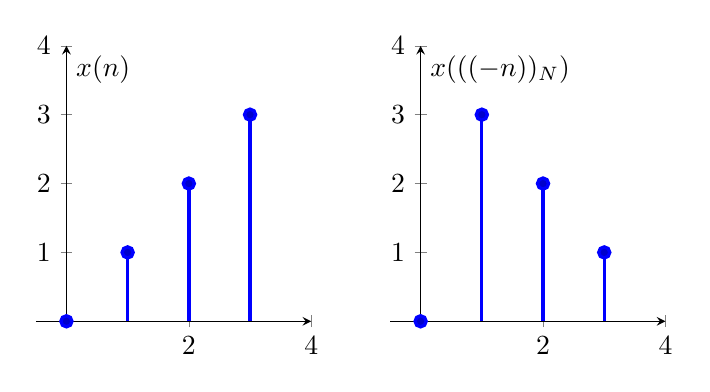
\begin{tikzpicture}
    \begin{groupplot}[
        group style={group size=2 by 1},
        axis lines=middle,
        width=2in,
        height=2in,
        ymax=4]
      \nextgroupplot[ylabel=$x(n)$, xmin=-0.5, xmax=4];
      \addplot+[ycomb, line width=1.2pt] plot coordinates {(0, 0) (1, 1) (2, 2) (3, 3)};
      \nextgroupplot[ylabel=$x(((-n))_N)$, xmin=-0.5, xmax=4];
      \addplot+[ycomb, line width=1.2pt] plot coordinates {(0, 0) (1, 3) (2, 2) (3, 1)};
    \end{groupplot}
  \end{tikzpicture}
  \caption{A circular shift}
\end{figure}
A circular convolution is equivalent to a periodic convolution over a single period.
\subsubsection{Linear Convolution with the DFT}
Because multiplying DFT coefficients performs a convolution, it turns out that we can compute a linear convolution using the circular convolution.
\begin{align*}
  x[n] \qquad 0\le n\le L-1\\
  h[n] \qquad 0 \le n \le P-1
\end{align*}
The linear convolution of these two signals will be length $L+P-1$, so in order to take an IDFT and get $L+P-1$ samples, we need to
take at least $N\le L+P-1$ points.
\begin{itemize}
  \item[1.] Pad each vector to length $L+P-1$
  \item[2.] Compute $X[k]H[k]$
  \item[3.] Take the Inverse DFT
\end{itemize}
If $N$ is too small, the result is akin to aliasing in the time domain.
To see why, consider that the DFT coefficients are essentially the DFS coefficients of the periodic extension of $x[n]$
$$\tilde{x}[n]=\sum_{r=-\infty}^{\infty}x[n-rN]$$
If we compute the DTFT of each periodic extension, then
$$Y(e^{j\omega})=X(e^{j\omega})H(e^{j\omega})$$ and the IDTFT of this will be
$$\tilde{y}[n] = \sum_{r=-\infty}^{\infty}y[n-rN]$$
Notice that if $N$ is not large enough, then these copies will be overlapping (a.k.a aliasing).
Since the DFT is just sampling the DTFT, the circular convolution will represent the true convolution
so long as the copies don't overlap.
\subsubsection{Block Convolutions}
In a discrete time system, the input signal might have a very long length, making it impractical to be stored in a computer's memory
or to compute the DFT of it all at once (especially if we have a real-time system). To compute the output of the filter (with impulse response of length $P$), we need to compute
the DFT in blocks shorter than the signal. \\\\The first method of block convolution is the overlap-add method.
\begin{itemize}
  \item[1.] Decompose $x[n]$ into nonoverlapping segments of length $L$
  \[ x_r[n] =
    \begin{cases}
      x[n] & rL \le n \le (r+1)L\\
      0 & \text{else}
    \end{cases}
  \]
  $$x[n] = \sum_{r}x_r[n]$$
  \item[2.] Since convolution is linear
  $$y[n] = x[n]*h[n]=\sum_r{x_r[n]*h[n]}$$
  \item[3.] Zero pad $x_r[n]$ and $h[n]$ to length $N\ge L+P-1$
  \item[4.] Compute the DFTs, multiply them, and take the inverse.
  \item[5.] The neighboring outputs overlap $P-1$, add the overlapping sections together to get the final output  
\end{itemize}
The other method of block convolution is the overlap-save method.
\begin{itemize}
  \item[1.] Divide $x[n]$ into sections of length $L$ such that each section overlaps the previous by $P-1$ points
  $$x_r[n]=x[n+r(L-P+1)-P+1] \qquad 0 \le n \le L-1$$
  \item[2.] Zero pad $x_r[n]$ and $h[n]$ to length $N\ge L+P-1$
  \item[3.] Compute the DFTs, multiply the coefficients, and compute the inverse.
  \item[4.] The first $P-1$ samples of the output will be incorrect, so we can discard them.
  $$y[n]=\sum_{r=0}^{\infty}y_r[n-r(L-P+1)+P-1]$$
  \[
    y_r[n]=
    \begin{cases}
      x_r[n]*h[n] & P-1\le n \le L-1\\
      0 & \text{ else}
    \end{cases}
  \]
\end{itemize}
\subsection{FFT}
The DFT gives us an easy way to do convolutions. Unfortunately, computing it is an $O(N^2)$ operation
because we must sum together $N$ elements to compute $N$ different coefficients. Thankfully, there is a fast
algorithm which can compute the DFT in $O(N\log N)$ time so we can compute convolutions quickly. The \textbf{Fast Fourier Transform}
is the algorithm which enables us to compute the DFT efficiently by exploiting properties of the Nth roots of unity.
$$W_N=e^{-j\frac{2\pi}{N}}$$
The roots of unity have the following properties:
\begin{align*}
  \textbf{Conjugate Symmetry: }& W_N^{N-n} = W_N^{-kn} = (W_N^{kn})^\star\\
  \textbf{Periodicity in N: }& W_{kn} = W_N^{k(n+N)} = W_N^{(k+N)n}\\
  \textbf{Power: } & W_N^2 = W_\frac{N}{2}
\end{align*}
There are two approaches to the FFT: decimation in time, which splits $x[n]$ into smaller subsequences, and decimation in frequency
which splits $X[n]$ into smaller subsequences.
\subsubsection{Decimation in Time}
The idea here is too break $x[n]$ into smaller subsequences. We assume that $N$ is a power of 2 for simplicity.
\begin{align*}
  X[k]=\sum_{n=0}^{N-1}x[n]W_N^{kn} = \sum_{\text{n even}}x[n]W_N^{kn}+\sum_{\text{n odd}}x[n]W_N^{kn}
\end{align*}
We let $n=2r$ and $n=2r+1$.
\begin{align*}
  X[k] &= \sum_{r=0}^{\frac{N}{2}-1}x[2r]W_N^{2rk}+\sum_{r=0}^{\frac{N}{2}-1}x[2r+1]W_N^{k(2r+1)}\\
  &= \sum_{r=0}^{\frac{N}{2}-1}x[2r]W_{\frac{N}{2}}^{rk}+W_N^k\sum_{r=0}^{\frac{N}{2}-1}x[2r+1]W_{\frac{N}{2}}^{kr}\\
\end{align*}
These are just the DFTs of the even and odd elements of the signal!
\begin{align*}
  \therefore X[k] = G[k] + W_N^kH[k]
\end{align*}
Both $G$ and $H$ are $\frac{N}{2}$ periodic, and notice that
$$W_N^{k+\frac{N}{2}}=e^{-j\frac{2\pi}{N}(k+\frac{N}{2})}= -W_N^k$$
This means once we compute $G[k]$ and $H[k]$ we can compute $X[k]$ easily because
$$X[k] = G[k]+W_N^kH[k]\qquad X\left[k+\frac{N}{2}\right]=G[k]-W_N^kH[k] \qquad \text{for }k\in\left[0, \frac{N}{2}\right)$$
We can continue this relationship recursively downwards.
Once we get too $N=2$, we can represet this as a simple butterfly operation.
$$X[0] = x[0]+x[1] \qquad X[1] = X[0]-X[1]$$
\subsubsection{Decimation in Frequency}
The decimation in frequency approach is very similar to the decimation in time approach except instead we split the frequency components
\begin{align*}
  X[2r] &= \sum_{n=0}^{\frac{N}{2}-1}x[n]W_N^{2rn}+\sum_{n=0}^{\frac{N}{2}-1}x\left[n+\frac{N}{2}\right]W_N^{2r\left(n+\frac{N}{2}\right)}=W_{\frac{N}{2}}^{rn}\sum_{n=0}^{\frac{N}{2}-1}\left(x[n]+x\left[n+\frac{N}{2}\right]\right)\\
  X[2r+1] &= W_{\frac{N}{2}}^{rn}\sum_{n=0}^{\frac{N}{2}-1}\left(x[n]-x\left[n+\frac{N}{2}\right]\right)
\end{align*}
\section{Spectral Analysis}
\begin{figure}[H]
  \centering
  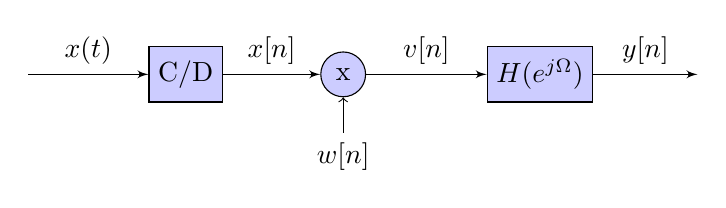
\begin{tikzpicture}[node distance=2.5cm,auto,>=latex']
      \node [int] (a) {C/D};
      \node (b) [left of=a,node distance=2cm, coordinate] {x(t)};
      \node [sum, pin={[init]below:$w[n]$}] (c) [right of=a, node distance=2cm] {x};
      \node [int] (d) [right of=c] {$H(e^{j\Omega})$};
      \node [coordinate] (end) [right of=d, node distance=2cm]{};
      \path[->] (b) edge node {$x(t)$} (a);
      \path[->] (a) edge node {$x[n]$} (c);
      \draw[->] (c) edge node {$v[n]$} (d) ;
      \draw[->] (d) edge node {$y[n]$} (end) ;
  \end{tikzpicture}    
\end{figure}
In real-world DSP systems, we are often converting a continuous time signal into a discrete one via sampling.
Because input is constantly streaming in, we can't process all of it at once, especially for real-time applications.
That is why we instead process blocks of length $L$ at a time. This is accomplished by multiplying by a window function $w[n]$.

All window functions are real, even, and finite. This means they have real and symmetric DTFTs. The most simply window is a box window (a sinc in the frequency domain).
When the signal is multiplied by a window, it amounts to a periodic convolution in the frequency domain
$$V(e^{j\Omega})=\frac{1}{2\pi}\int_{\langle 2\pi \rangle}X(e^{j\Omega})W(e^{j(\Omega-\omega)})d\omega$$
This periodic convolution means our choice of window function has an impact on our ability to resolve frequencies in the frequency domain.
\begin{itemize}
  \item If $W(e^{j\Omega})$ has a wide "main lobe" at the DC frequencies, then the spectrum of $V(e^{j\Omega})$ will be blurred
  \item If $W(e^{j\Omega})$ has large "side lobes" at non DC frequencies, then \textbf{spectral leakage} occurs because larger frequencies start bleeding into lower ones.
\end{itemize}
Another factor which impacts our ability to resolve frequencies in frequency domain is the length of the window. Because an L point DFT samples the DTFT at L points,
taking a larger window will resolve the DTFT better. If we don't want too increase the window length (because doing so would decrease the latency of our system), we can
zero pad after windowing because zero padding has no length on the DFT.
$$\sum_{n=0}^{N-1}{v[n]W_n^k} = \sum_{n=0}^{L-1}{v[n]W_n^k}\qquad \text{ if } \forall L<n<N-1,v[n]=0$$
\subsection{Short Time Fourier Transform (STFT)}
An important part of Spectral Analysis is understanding the frequencies present in a signal. However, by looking at the DFT of a signal $x[n]$, we only get the frequency information
across the entire duration of the signal. Likewise, just by looking at $x[n]$, we get no frequency information and only temporal information. The STFT is a tool to see both at once.
$$X[n, \omega) = \sum_{m=-\infty}^{\infty}x[n+m]w[m]e^{j\omega m}$$
essentially, we slide a window function around x and compute the DTFT at every time point. This creates a map from 1 dimension to 2D. This map is called the spectrogram.
In the STFT, $\omega$ is continuous while $n$ is discrete.
\subsection{Discrete STFT}
Just like the DFT discretizes the DTFT, we can make the STFT purely discrete with the DSTFT.
$$X[r, k] = \sum_{m=0}^{L-1}x[rR+m]w[m]W_N^{km}$$
Just like before, we take our window and slide it around the signal, computing DFTs at every time point.
Our window is of length $L$, $R$ is how much we shift the window around, and $N \ge L$ is the DFT length we are taking.
If $N > L$, then we are essentially computing a zero-padded DFT. This produces a spectrogram which we can display digitally.
To reconstruct the signal from the DSTFT
$$x[rR+m]w_L[m] = \frac{1}{N}\sum_{k=0}^{N-1}X[n, k]W_N^{-km}$$
As long as the window is not 0 and the windows don't overlap, $$x[n] = \frac{x[n-rL]}{w_L[n-rL]}$$
\subsection{Time-Frequency Uncertainty} 
When we compute the spectrogram of a signal, we can think of each coefficient as "tiling" the time-frequency space.
If we consider the normal N point DFT, each DFT coefficient is supported by N points in the time domain. Since the DFT samples the DTFT, it divides the range of $[0, 2\pi]$
into $N$ segments of width $\frac{2\pi}{N}$. Each coefficient represents one of these coefficients, leading to a tiling looking like this (for a 5 point DFT).
\begin{figure}[H]
  \centering
  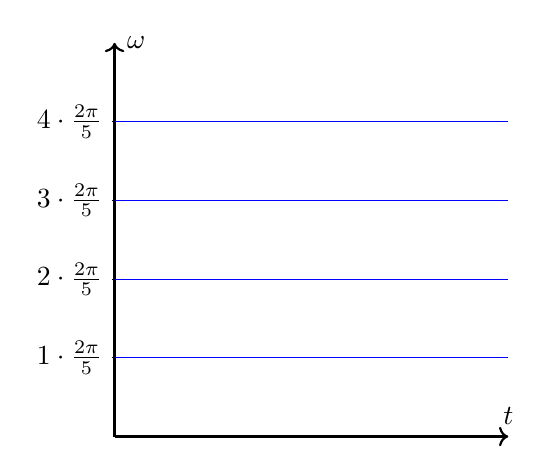
\begin{tikzpicture}
      \draw[thick,->] (0, 0) -- (5,0);
      \draw[thick,->] (0,0) -- (0,5);
      \draw (5 cm,1pt) node[anchor=south] {$t$};
      \draw (1pt,5cm) node[anchor=west] {$\omega$};
      \foreach \y in {1, 2, 3, 4}
          \draw (1pt,\y cm) -- (-1pt,\y cm) node[anchor=east] {$\y\cdot \frac{2\pi}{5}$};
      \draw[scale=1,domain=0:5,smooth,variable=\x,blue] plot ({\x},{1});
      \draw[scale=1,domain=0:5,smooth,variable=\x,blue] plot ({\x},{2});
      \draw[scale=1,domain=0:5,smooth,variable=\x,blue] plot ({\x},{3});
      \draw[scale=1,domain=0:5,smooth,variable=\x,blue] plot ({\x},{4});
  \end{tikzpicture}  
\end{figure}
Thinking about the DSTFT, each coefficient is computed using $L$ points of the original signal. Each coefficient
still represents intervals of $\frac{2\pi}{N}$ in the frequency axis. This leads to a tiling which looks like this.
\begin{figure}[H]
  \centering
  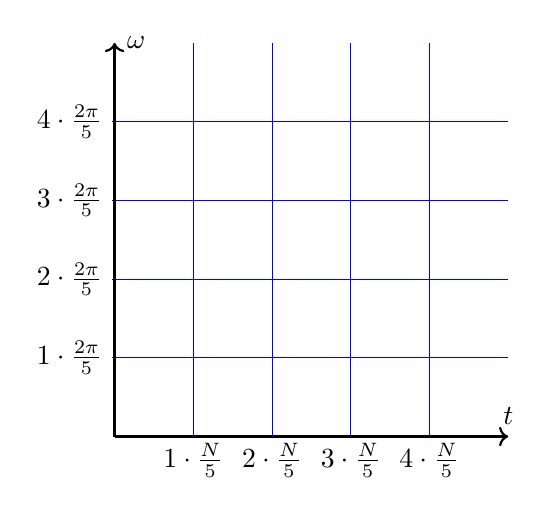
\begin{tikzpicture}
      \draw[thick,->] (0, 0) -- (5,0);
      \draw[thick,->] (0,0) -- (0,5);
      \draw (5 cm,1pt) node[anchor=south] {$t$};
      \draw (1pt,5cm) node[anchor=west] {$\omega$};
      \foreach \y in {1, 2, 3, 4} {
          \draw (1pt,\y cm) -- (-1pt,\y cm) node[anchor=east] {$\y\cdot \frac{2\pi}{5}$};
          \draw[scale=1,domain=0:5,smooth,variable=\x,blue] plot ({\x},{\y});
      }
      \foreach \x in {1, 2, 3, 4} {
          \draw (\x cm, 1pt) -- (\x cm, 1pt) node[anchor=north] {$\x\cdot \frac{N}{5}$};
          \draw[scale=1,domain=0:5,smooth,variable=\y,blue] plot ({\x},{\y});
      }
  \end{tikzpicture}  
\end{figure}
What these tilings show us is that because we have discretized time and frequency,
there is some uncertainty regarding which times and frequencies each coefficient represents.

We can formalize this idea by considering a general transform. All transforms are really an inner product with a set of basis functions
$$T_x(\gamma) = \langle x(t), \phi_\gamma(t) \rangle=\int_{-\infty}^{\infty}x(t)\phi_\gamma^\star(t)dt$$
For each particular $\gamma$, that $T_x(\gamma)$ is the projection of our signal onto the basis vector $\phi_\gamma(t)$. We can use Parseval's relationship
to see that
\begin{align*}
  T_x(\gamma) &= \langle x(t), \phi_\gamma(t) \rangle =\int_{-\infty}^{\infty}x(t)\phi_\gamma^\star(t)dt \\
  &= \frac{1}{2\pi}\int_{-\infty}^{\infty}X(j\Omega)\Phi_\gamma^\star(j\Omega)d\Omega \\
  &= \langle X(j\Omega), \frac{1}{2\pi}\Phi_\lambda(j\Omega)\rangle
\end{align*}
This means that we can equivalently think of projecting the spectrum of our signal onto the spectrum of our basis function. Remember that projection essentially asks "How much of a signal can be explained by the basis".
We can formalize this by looking at the signal in a statistical sense and treat it as a probability distribution.
\begin{align*}
  m_t &= \int_{-\infty}^{\infty}t|\psi(t)|^2dt &\qquad m_\Omega &= \int_{-\infty}^{\infty}\Omega\frac{1}{2\pi}|\Psi(j\Omega)|^2d\Omega\\
  \sigma_t^2 &= \int_{-\infty}^{\infty}(t-m_t)^2|\psi(t)|^2dt &\qquad \sigma^2_\Omega &= \int_{-\infty}^{\infty}(\Omega-m_\Omega)^2\frac{1}{2\pi}|\Psi(j\Omega)|^2d\Omega\\
\end{align*}
$m_t$ and $m_\Omega$ are the means of the signal and the spectrum. $\sigma_t^2$ and $\sigma_\Omega^2$ are the variances. Together, they localize where our signal "lives" in the time-frequency spectrum.
The uncertainty principle says
$$\sigma_t\sigma_w \ge \frac{1}{2}$$
This means there is nothing we can do to get completely accurate time resolution and frequency resolution, and any decisions we make will
lead to a tradeoff between them.
\subsection{Wavelets}
While the STFT gives us a better picture of a signal than a full-length DFT, one of its shortcomings is that each coefficient is supported by the same amount of time and frequency. Low frequencies don't change as
much as high frequencies do, so a lower frequency needs to be resolved with more time support whereas a fast signal would requires less time support to resolve properly.
The Wavelet transform takes this idea and tiles the Time-Frequency spectrum with different time and frequency supports (essentially making all of the boxes different sizes) by using a scaled bandpass filter $\Psi(t)$ as its kernel.
$$\int_{-\infty}^{\infty}|\Psi(t)|^2dt=1 \qquad \int_{-\infty}^{\infty}\Psi(t)dt = 0$$
This kernel is called the mother wavelet. The continuous wavelet transform then becomes.
$$Wf(u, s) = \int_{-\infty}^{\infty}f(t)\frac{1}{\sqrt{s}}\Psi^\star\left(\frac{t-u}{s}\right)dt$$
We need an infinite number of functins to fully represent all frequencies properly, but at a certain level, we don't care about our ability to resolve them better, so we stop scaling and
use a low frequency function $\Phi(t)$ to "plug" the remaining bandwidth. this is called the "father" wavelet.
\subsubsection{Discrete Wavelet Transform}
In discrete time, the wavelet transform becomes
$$d_{s,u}=\sum_{n=0}^{N-1}x[n]\Psi_{s,u}[n] \qquad a_{s,u}=\sum_{n=0}^{N-1}x[n]\Phi_{s,u}[n]$$
The $d$ coefficients are the detailed coefficients and are computed using the mother wavelet. The capture higher frequency information.
The $a$ coefficients are the approximate coefficients computed using the father wavelet. They represent lower frequency information.
The time frequency tiling for the DWT looks something like this.
\begin{figure}[H]
  \centering
  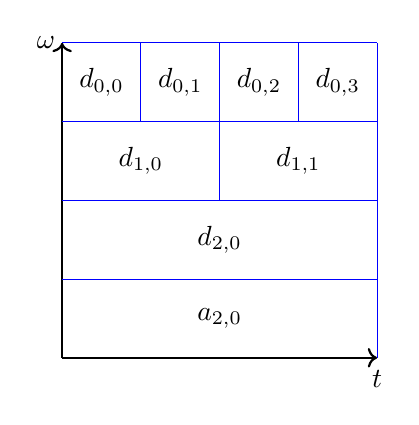
\begin{tikzpicture}
      \draw[thick,->] (0, 0) -- (4,0);
      \draw[thick,->] (0,0) -- (0,4);
      \draw (4 cm,-1pt) node[anchor=north] {$t$};
      \draw (1pt,4cm) node[anchor=east] {$\omega$};
      \foreach \y in {1, 2, 3, 4} {
          \draw[scale=1,domain=0:4,smooth,variable=\x,blue] plot ({\x},{\y});
      }
      \foreach \x in {1, 2, 3} {
          \draw[scale=1,domain=3:4,smooth,variable=\y,blue] plot ({\x},{\y});
      }
      \draw[scale=1,domain=0:4,smooth,variable=\y,blue] plot ({4},{\y});
      \draw[scale=1,domain=2:3,smooth,variable=\y,blue] plot ({2},{\y});
      \draw (0.5cm,3.5cm) node[] {$d_{0,0}$};
      \draw (1.5cm,3.5cm) node[] {$d_{0,1}$};
      \draw (2.5cm,3.5cm) node[] {$d_{0,2}$};
      \draw (3.5cm,3.5cm) node[] {$d_{0,3}$};
      \draw (1cm,2.5cm) node[] {$d_{1,0}$};
      \draw (3cm,2.5cm) node[] {$d_{1,1}$};
      \draw (2cm,1.5cm) node[] {$d_{2,0}$};
      \draw (2cm,0.5cm) node[] {$a_{2,0}$};
  \end{tikzpicture}  
\end{figure}
Notice how each Wavelet coefficient is supported by a different amount of time and frequency.
We can choose different mother and father wavelets to describe our signals. For example, the Haar wavelet
does very well with piecewise constant signals.
\section{Sampling}
\subsection{Ideal Sampling}
In order to work with continuous signals using a computer, we need to sample them. This means recording the value at particular points of time.
During uniform sampling, we take samples at an even sampling period $T_s$ so $x[n]=x_c(nT)$. This is done by passing the signal through an Analog-To-Digital converter.
From there we can do discrete time processing and reconstruct our signal by passing it through a Digital-to-Analog converter with reconstruction period $T_r$.
\begin{figure}[H]
  \centering
  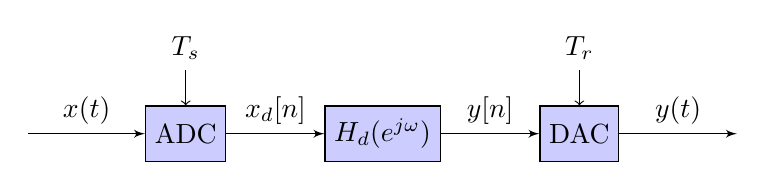
\begin{tikzpicture}[node distance=2.5cm,auto,>=latex']
      \node [int, pin={[init]above:$T_s$}] (a) {ADC};
      \node (b) [left of=a,node distance=2cm, coordinate] {x(t)};
      \node [int] (c) [right of=a] {$H_d(e^{j\omega})$};
      \node [int, pin={[init]above:$T_r$}] (d) [right of=c] {DAC};
      \node [coordinate] (end) [right of=d, node distance=2cm]{};
      \path[->] (b) edge node {$x(t)$} (a);
      \path[->] (a) edge node {$x_d[n]$} (c);
      \draw[->] (c) edge node {$y[n]$} (d) ;
      \draw[->] (d) edge node {$y(t)$} (end) ;
  \end{tikzpicture}    
\end{figure}
We mathematically model sampling as multiplication by an impulse train. Notice that if we were to take a signal $x(t)$ and multiply it by an impulse train, then we would get a series of impulses
equal to $x(t)$ at the sampling points and $0$ everywhere else. We can call this signal $x_p(t)$.
$$p(t) = \sum_{k=-\infty}^{\infty}{\delta(t-kT)}$$
$$x_p(t) = x(t)p(t) = \sum_{k=-\infty}^{\infty}{x(t)\delta(t-kT)}$$
In the Fourier Domain,
\begin{align*}
    X_p(j\Omega) &= \frac{1}{2\pi}X(j\Omega)*P(j\Omega)\\
    P(j\Omega) &= \frac{2\pi}{T}\sum_{k=-\infty}^{\infty}{\delta(\Omega-k\Omega_s)}\\
    \therefore X_p(j\Omega) &= \frac{1}{2\pi}\int_{-\infty}^{\infty}{X(j\theta)P(j(\Omega-\theta))d\theta} = \frac{1}{T}\sum_{k=-\infty}^{\infty}{X(j(\Omega-k\Omega_s)}
\end{align*}
What this tells us is that the Fourier Transform of our sampled signal is a series of copies of $X(j\Omega)$, each centered
at $k\Omega_s$ where $\Omega_s = \frac{2\pi}{T}$. This is a good model because we can equivalently write the CTFT of the impulse train sampled signal as
\begin{align*}
  X_p(j\Omega) &= \int_{-\infty}^{\infty}\sum_{k=-\infty}^{\infty}{x(t)\delta(t-kT)} \sum_{k=-\infty}^{\infty}x(kT)e^{-jkT\Omega} 
\end{align*}
Notice that this is just the DTFT of $x[n]=x(nT)$ if we set $\omega = \Omega T$
$$X(e^{j\omega}) = \sum_{n=-\infty}^{\infty}x(nT)e^{-j\omega n}=X_p(j\Omega)|_{\Omega=\frac{\omega}{T}}=\frac{1}{T}\sum_{k=-\infty}^{\infty}{X\left(\frac{\omega}{T}-k\frac{2\pi}{T_s}\right)}$$
This means that the DTFT of our signal is just a bunch of shifted copies, and the frequency axis is scaled so $\Omega_s \rightarrow 2\pi$.
\subsubsection{Nyquist Theorem}
To analyze this further, we will stay in continuous time. Lets say that our original signal has the following Fourier Transform. Notice the signal is band-limited by $\Omega_M$.
\begin{figure}[H]
    \centering
    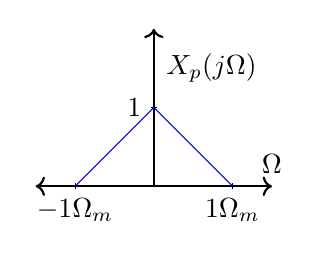
\begin{tikzpicture}
        \draw[thick,<->] (-1.5, 0) -- (1.5,0);
        \draw[thick,->] (0,0) -- (0,2);
        \draw (1.5 cm,1pt) node[anchor=south] {$\Omega$};
        \draw (1pt,1.5cm) node[anchor=west] {$X_p(j\Omega)$};
        \foreach \x in {-1,1}
            \draw (\x cm,1pt) -- (\x cm,-1pt) node[anchor=north] {$\x\Omega_m$};
        \foreach \y in {1}
            \draw (1pt,\y cm) -- (-1pt,\y cm) node[anchor=east] {$\y$};
            \draw[scale=1,domain=0:1,smooth,variable=\x,blue] plot ({\x},{1-\x});
            \draw[scale=1,domain=-1:0,smooth,variable=\x,blue] plot ({\x},{\x+1});
    \end{tikzpicture}  
\end{figure}
There are two major cases: if $\Omega_s > 2\Omega_m$ and $\Omega_s < 2\Omega_m$.\\
\textbf{Case One: }$\Omega_s > 2\Omega_m$
\begin{figure}[H]
    \centering
    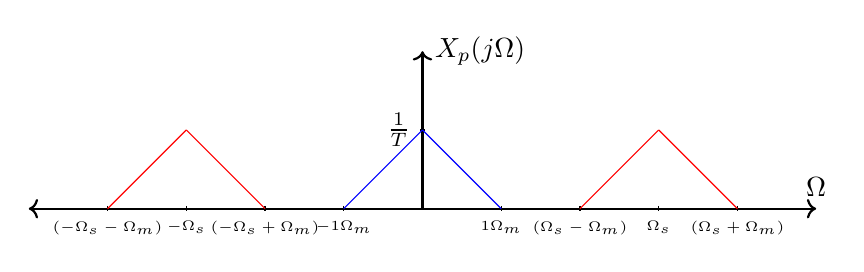
\begin{tikzpicture}
        \draw[thick,<->] (-5, 0) -- (5,0);
        \draw[thick,->] (0,0) -- (0,2);
        \draw (5 cm,1pt) node[anchor=south] {$\Omega$};
        \draw (1pt,2cm) node[anchor=west] {$X_p(j\Omega)$};
        \draw (3 cm,1pt) -- (3 cm,-1pt) node[anchor=north, font=\tiny] {$\Omega_s$};
        \draw (-3 cm,1pt) -- (-3 cm,-1pt) node[anchor=north, font=\tiny] {$-\Omega_s$};
        \draw (2 cm,1pt) -- (2 cm,-1pt) node[anchor=north, font=\tiny] {$(\Omega_s-\Omega_m)$};
        \draw (4 cm,1pt) -- (4 cm,-1pt) node[anchor=north, font=\tiny] {$(\Omega_s+\Omega_m)$};
        \draw (-2 cm,1pt) -- (-2 cm,-1pt) node[anchor=north, font=\tiny] {$(-\Omega_s+\Omega_m)$};
        \draw (-4 cm,1pt) -- (-4 cm,-1pt) node[anchor=north, font=\tiny] {$(-\Omega_s-\Omega_m)$};
        \foreach \x in {-1,1}
            \draw (\x cm,1pt) -- (\x cm,-1pt) node[anchor=north, font=\tiny] {$\x\Omega_m$};
        \foreach \y in {1}
            \draw (1pt,\y cm) -- (-1pt,\y cm) node[anchor=east] {$\frac{\y}{T}$};
            \draw[scale=1,domain=0:1,smooth,variable=\x,blue] plot ({\x},{1-\x});
            \draw[scale=1,domain=-1:0,smooth,variable=\x,blue] plot ({\x},{\x+1});
            \draw[scale=1,domain=3:4,smooth,variable=\x,red] plot ({\x},{4-\x});
            \draw[scale=1,domain=2:3,smooth,variable=\x,red] plot ({\x},{\x-2});
            \draw[scale=1,domain=-4:-3,smooth,variable=\x,red] plot ({\x},{4+\x});
            \draw[scale=1,domain=-3:-2,smooth,variable=\x,red] plot ({\x},{-2-\x});
    \end{tikzpicture}  
\end{figure}
When $\Omega_s > 2\Omega_M$, the shifted copies of the original $X(j\Omega)$ (shown in blue)
do not overlap with each other or which the original copy. If we wanted to recover the original
signal, we could simply apply a low pass filter to isolate the unshifted copy of $X(j\Omega)$ and
then take the inverse Fourier Transform.\\
\textbf{Case Two: }$\Omega_s < 2\Omega_m$
\begin{figure}[H]
    \centering
    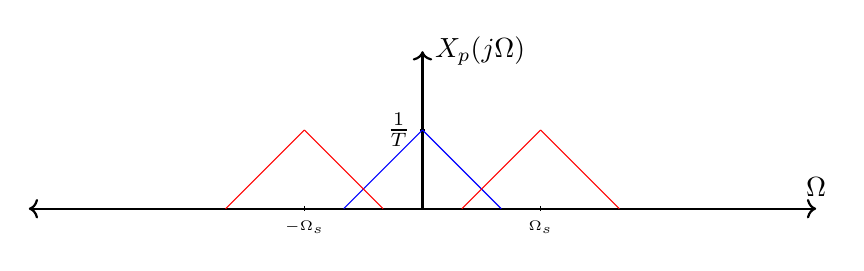
\begin{tikzpicture}
        \draw[thick,<->] (-5, 0) -- (5,0);
        \draw[thick,->] (0,0) -- (0,2);
        \draw (5 cm,1pt) node[anchor=south] {$\Omega$};
        \draw (1pt,2cm) node[anchor=west] {$X_p(j\Omega)$};
        \draw (1.5 cm,1pt) -- (1.5 cm,-1pt) node[anchor=north, font=\tiny] {$\Omega_s$};
        \draw (-1.5 cm,1pt) -- (-1.5 cm,-1pt) node[anchor=north, font=\tiny] {$-\Omega_s$};
        \foreach \y in {1}
            \draw (1pt,\y cm) -- (-1pt,\y cm) node[anchor=east] {$\frac{\y}{T}$};
            \draw[scale=1,domain=0:1,smooth,variable=\x,blue] plot ({\x},{1-\x});
            \draw[scale=1,domain=-1:0,smooth,variable=\x,blue] plot ({\x},{\x+1});
            \draw[scale=1,domain=1.5:2.5,smooth,variable=\x,red] plot ({\x},{2.5-\x});
            \draw[scale=1,domain=0.5:1.5,smooth,variable=\x,red] plot ({\x},{\x-0.5});
            \draw[scale=1,domain=-2.5:-1.5,smooth,variable=\x,red] plot ({\x},{2.5+\x});
            \draw[scale=1,domain=-1.5:-0.5,smooth,variable=\x,red] plot ({\x},{-0.5-\x});
    \end{tikzpicture}  
\end{figure}
Notice how in this case, the shifted copies overlap with the original $X(\omega)$. This means in our sampled signal, the higher frequency
information is bleeding in with the lower frequency information. This phenomenon is known as aliasing. When aliasing occurs, we cannot simply
apply a low pass filter to isolate the unshifted copy of $X(\omega)$.\\\\
When $\Omega_s = 2\Omega_M$, then our ability to reconstruct the original signal depends on the shape of its Fourier Transform. As long as $X_p(jk\Omega_m)$
are equal to $X(j\Omega_m)$ and $X(-j\Omega_m$), then we can apply an LPF because we can isolate the original $X(j\Omega)$ and take its inverse Fourier Transform.\\\\
Remember that an ideal low pass filter is a square wave in the frequency domain and a sinc in the time domain. Thus if we allow
\[
    X_r(j\Omega) = X_p(j\Omega)\cdot \left\{
            \begin{array}{cc}
                T & |\Omega| < \frac{\Omega_s}{2}\\
                0 & \text{ else }
            \end{array}
        \right\}
\]
then our reconstructed signal will be
$$x_r(t) = x_p(t)*sinc\left(\frac{t}{T}\right) = \sum_{n=-\infty}^{\infty}{X(nT)sinc\left(\frac{t-nT}{T}\right)}$$
This is why we call reconstructing a signal from its samples "sinc interpolation."
This leads us to formulate the Nyquist Theorem.
\begin{theorem}[Nyquist Theorem]
    Suppose a continuous signal $x$ is bandlimited and we sample it at a rate of $\Omega_s > 2\Omega_m$, then the signal $x_r(t)$
    reconstructed by sinc interpolation is exactly $x(t)$
\end{theorem}
\subsubsection{Discrete Time Processing of a Continuous Time Signal}
As long as the DT system we apply is LTI, the overall CT system will be linear too, but it will not necessarily be time invariant
because sampling inherently depends on the signal's timing.
\begin{figure}[H]
  \centering
  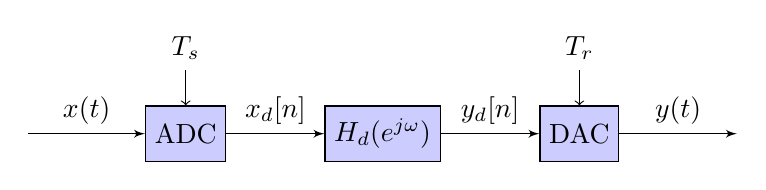
\begin{tikzpicture}[node distance=2.5cm,auto,>=latex']
      \node [int, pin={[init]above:$T_s$}] (a) {ADC};
      \node (b) [left of=a,node distance=2cm, coordinate] {x(t)};
      \node [int] (c) [right of=a] {$H_d(e^{j\omega})$};
      \node [int, pin={[init]above:$T_r$}] (d) [right of=c] {DAC};
      \node [coordinate] (end) [right of=d, node distance=2cm]{};
      \path[->] (b) edge node {$x(t)$} (a);
      \path[->] (a) edge node {$x_d[n]$} (c);
      \draw[->] (c) edge node {$y_d[n]$} (d) ;
      \draw[->] (d) edge node {$y(t)$} (end) ;
  \end{tikzpicture}    
\end{figure}
If we want to find the overall CT transfer function ($\omega = \Omega T$)
\begin{align*}
    Y_d(e^{j\omega}) &= H_d(e^{j\omega})X_d(e^{j\omega}) = H_d(e^{j\omega})X_p\left(\frac{\omega}{T}\right)\\
    Y_p(j\Omega) &= Y_d(e^{j\Omega T}) = H_d(e^{j\Omega T})X_p(j\Omega)\\
    Y(j\Omega) &= \left\{
        \begin{array}{cc}
            T & |\Omega| < \frac{\Omega_s}{2}\\
            0 & |\Omega| \ge \frac{\Omega_s}{2}
        \end{array}
        \right\} \cdot Y_p(j\Omega) = \left\{
            \begin{array}{cc}
                TH_d(e^{j\Omega T})X_p(j\Omega) & |\Omega| < \frac{\Omega_s}{2}\\
                0 & |\Omega| \ge \frac{\Omega_s}{2}
            \end{array}
            \right\}
\end{align*}
Assuming that the Nyquist theorem holds,
\begin{align*}
    X_p(j\Omega) &= \frac{1}{T}X(j\Omega)\\
    \therefore Y(j\Omega) &= \left\{
        \begin{array}{cc}
            H_d(e^{j\Omega T})X(j\omega) & |\Omega| < \frac{\Omega_s}{2}\\
            0 & |\Omega| \ge \frac{\Omega_s}{2}
        \end{array}
    \right\}\\
        \therefore H_{system} &= \left\{\begin{array}{cc}
            H_d(e^{j\omega T}) & |\Omega| < \frac{\Omega_s}{2}\\
            0 & |\Omega| \ge \frac{\Omega_s}{2}
        \end{array}
        \right\}
\end{align*}
This shows us that as long as the Nyquist theorem holds, we can process continuous signals
with a disrete time LTI system and still have the result be LTI.
\subsubsection{Continuous Time Processing of Discrete Time Signals}
While not useful in practice, it can be useful to model a discrete time transfer function in terms of Continuous Time processing (e.g a half sample delay).
\begin{figure}[H]
  \centering
  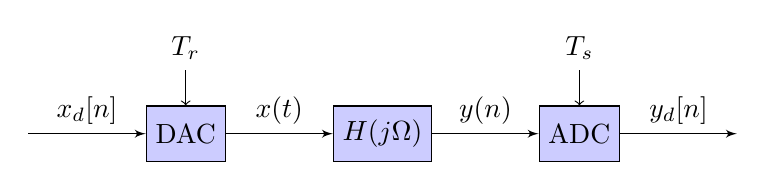
\begin{tikzpicture}[node distance=2.5cm,auto,>=latex']
      \node [int, pin={[init]above:$T_r$}] (a) {DAC};
      \node (b) [left of=a,node distance=2cm, coordinate] {x(t)};
      \node [int] (c) [right of=a] {$H(j\Omega)$};
      \node [int, pin={[init]above:$T_s$}] (d) [right of=c] {ADC};
      \node [coordinate] (end) [right of=d, node distance=2cm]{};
      \path[->] (b) edge node {$x_d[n]$} (a);
      \path[->] (a) edge node {$x(t)$} (c);
      \draw[->] (c) edge node {$y(n)$} (d) ;
      \draw[->] (d) edge node {$y_d[n]$} (end) ;
  \end{tikzpicture}    
\end{figure}
Similar to the analysis of DT processing of a CT signal, we can write the discrete transfer function in terms of the continuous function.
Our continuous signal will be bandlimited after reconstruction.
\[
  X(j\Omega) = \begin{cases}
    T X_d(e^{j\omega})|_{\omega=\Omega T} & |\Omega| \le \frac{\Omega_s}{2}\\
    0
  \end{cases}
\]
This means our reconstructed signal $Y(j\Omega)=H_(j\Omega)X(j\Omega)$ is also bandlimited, so we can say that
$$Y_d(e^{j\Omega})=H(j\Omega)|_{\Omega=\frac{\omega}{T}}X(e^{j\omega})$$
\subsubsection{Downsampling}
When we downsample a signal by a factor of $M$, we create a new signal $y[n]=x[nM]$ by taking every $Mth$ sample. What this means conceptually is that we are reconstructing the continuous signal
and then sampling it at a slower rate $MT$ where $T$ was the original sampling rate. If $x_c$ is the original continuous time signal and $x_d$ is the sampled signal, then the downsampled signal $y[n]$
will be
$$y[n]=x[nM]=x_c(nMT)\implies Y(e^{j\omega}) =\frac{1}{MT}\sum_{k=-\infty}^{\infty}X_c\left(\frac{\omega}{NT}-k\frac{2\pi}{NT}\right)$$
If we re-index and let $k=Mp+m$ for $m\in [0, N-1],p\in \mathbb{Z}$
$$Y(e^{j\omega})=\frac{1}{M}\sum_{m=0}^{M-1}X_d(e^{j\frac{\omega-2\pi m}{M}})$$
What this means is to obtain the new DTFT, we need to scale the frequency axis so $\frac{\pi}{M}\rightarrow \pi$.
To prevent aliasing when this happens, we include an LPF before the downsample step.
\begin{figure}[H]
  \centering
  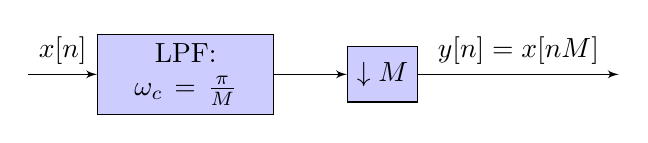
\begin{tikzpicture}[node distance=2.5cm,auto,>=latex']
      \node [int, text width=2cm, align=center] (a) {LPF:\\$\omega_c=\frac{\pi}{M}$};
      \node (b) [left of=a,node distance=2cm, coordinate] {x(t)};
      \node [int] (c) [right of=a] {$\downarrow M$};
      \node [coordinate] (end) [right of=c, node distance=3cm]{};
      \path[->] (b) edge node {$x[n]$} (a);
      \path[->] (a) edge node {} (c);
      \draw[->] (c) edge node {$y[n]=x[nM]$} (end);
  \end{tikzpicture}    
\end{figure}
\subsubsection{Upsampling}
When we upsample a signal by a factor of L, we are interpolating between samples. Conceptually, this means we are
reconstructing the original continuous time signal and resampling it at a faster rate than before.
First we place zeros in between samples, effectively expanding our signal.
\[
  x_e[n] = \begin{cases}
    x\left[\frac{n}{L}\right] & n=0, \pm L, \pm 2L,...\\
    0
  \end{cases}
\]
$$X_e(e^{j\omega})=\sum_{-\infty}^{\infty}x_e[n]e^{-j\omega n}=\sum_{m=-\infty}^{\infty}x[m]e^{-j\omega mL} = X\left(e^{j\omega L}\right)$$
Then we interpolate by convolving with a sinc.
$$y[n] = x_e[n]*sinc\left(\frac{n}{L}\right) = \sum_{n=-\infty}^{\infty}{x[k]sinc\left(\frac{n-kL}{L}\right)}$$
In the frequency domain, this looks like compressing the frequency axis so $\pi \rightarrow \frac{\pi}{L}$ and then taking a low pass filter.
\begin{figure}[H]
  \centering
  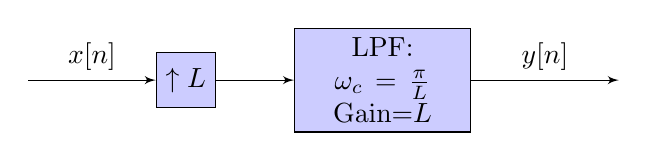
\begin{tikzpicture}[node distance=2.5cm,auto,>=latex']
      \node [int] (a) {$\uparrow L$};
      \node (b) [left of=a,node distance=2cm, coordinate] {x(t)};
      \node [int, text width=2cm, align=center] (c) [right of=a] {LPF:\\$\omega_c=\frac{\pi}{L}$\\Gain=$L$};
      \node [coordinate] (end) [right of=c, node distance=3cm]{};
      \path[->] (b) edge node {$x[n]$} (a);
      \path[->] (a) edge node {} (c);
      \draw[->] (c) edge node {$y[n]$} (end);
  \end{tikzpicture}    
\end{figure}
The gain of L is used to scale the spectrum so it is identical to if we had sampled the continuous signal at a rate of $\frac{T}{L}$.
\subsection{Multi-Rate Signal Processing}
In order to resample a signal to a rate $T'=\frac{MT}{L}$ where T is the original sampling rate, we can do this by upsampling then downsampling our signal.
\begin{figure}[H]
  \centering
  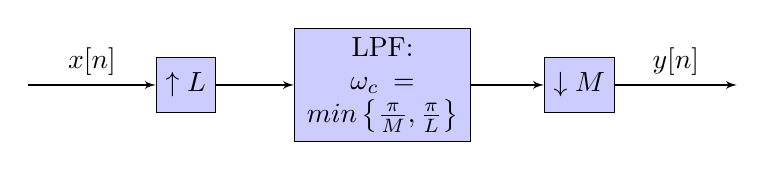
\begin{tikzpicture}[node distance=2.5cm,auto,>=latex']
      \node [int] (a) {$\uparrow L$};
      \node (b) [left of=a,node distance=2cm, coordinate] {x(t)};
      \node [filter] (c) [right of=a] {LPF:\\$\omega_c=min\left\{\frac{\pi}{M}, \frac{\pi}{L}\right\}$};
      \node [int] (d) [right of=c] {$\downarrow M$};
      \node [coordinate] (end) [right of=d, node distance=2cm]{};
      \path[->] (b) edge node {$x[n]$} (a);
      \path[->] (a) edge node {} (c);
      \path[->] (c) edge node {} (d);
      \draw[->] (d) edge node {$y[n]$} (end);
  \end{tikzpicture}    
\end{figure}
Notice that we only need one LPF to take care of both anti-aliasing and interpolation.
\subsubsection{Exchanging Filter Order During Resampling}
Notice that resampling with a very small change wastes a lot of computation. For example, resampling with $T'=1.01T$
would upsample by 100 and then throw away most of those samples when we downsample. Thus it would be useful to exchange the order of operations when resampling to save computation.
\begin{figure}[H]
  \centering
  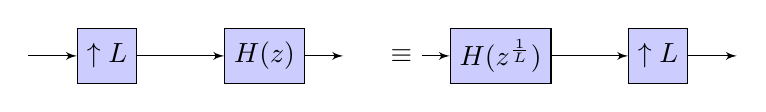
\begin{tikzpicture}[node distance=2cm,auto,>=latex']
      \node [int] (a) {$\uparrow L$};
      \node (b) [left of=a,node distance=1cm, coordinate] {x(t)};
      \node [int] (c) [right of=a] {$H(z)$};
      \node [coordinate] (end) [right of=c, node distance=1cm]{};
      \path[->] (b) edge node {} (a);
      \path[->] (a) edge node {} (c);
      \draw[->] (c) edge node {} (end);

      \node (y) [right of=end,node distance=1cm, coordinate] {x(t)};
      \draw[] (y) edge node {$\equiv$} (y);
            
      \node (e) [right of=c,node distance=2cm, coordinate] {x(t)};
      \node [int] (d) [right of=e, node distance=1cm]{$H(z^{\frac{1}{L}})$};
      \node [int] (f) [right of=d] {$\uparrow L$};
      \node [coordinate] (end2) [right of=f, node distance=1cm]{};
      \path[->] (e) edge node {} (d);
      \path[->] (d) edge node {} (f);
      \draw[->] (f) edge node {} (end2);
  \end{tikzpicture}    
\end{figure}
During upsampling, we convolve our filter with a bunch of zeros caused by the expansion. Convolution with 0's is a unnecessary, so instead we could convolve with a compressed version of the filter. Notice the results will be the same as long as $H(z^{\frac{1}{L}})$ is a rational function,
\begin{figure}[H]
  \centering
  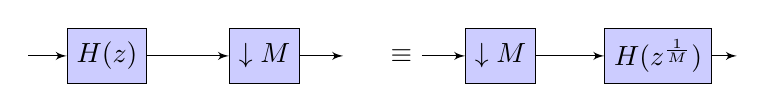
\begin{tikzpicture}[node distance=2cm,auto,>=latex']
      \node [int] (a) {$H(z)$};
      \node (b) [left of=a,node distance=1cm, coordinate] {x(t)};
      \node [int] (c) [right of=a] {$\downarrow M$};
      \node [coordinate] (end) [right of=c, node distance=1cm]{};
      \path[->] (b) edge node {} (a);
      \path[->] (a) edge node {} (c);
      \draw[->] (c) edge node {} (end);

      \node (y) [right of=end,node distance=1cm, coordinate] {x(t)};
      \draw[] (y) edge node {$\equiv$} (y);
            
      \node (e) [right of=c,node distance=2cm, coordinate] {x(t)};
      \node [int] (d) [right of=e, node distance=1cm]{$\downarrow M$};
      \node [int] (f) [right of=d] {$H(z^{\frac{1}{M}})$};
      \node [coordinate] (end2) [right of=f, node distance=1cm]{};
      \path[->] (e) edge node {} (d);
      \path[->] (d) edge node {} (f);
      \draw[->] (f) edge node {} (end2);
  \end{tikzpicture}    
\end{figure}
During downsampling, we do a convolution and then throw away most of our results. It would be much more efficient to instead compute only the quantities we need.
This is accomplished by downsmapling first and then convolving. Just like before, the results are only going to be the same if $H(z^{\frac{1}{M}})$ is a rational function.
\subsubsection{Polyphase Decomposition}
The problem with interchanging filters is that it is not always possible. Most filters are not compressible. However, we can get around this issue
and still get the efficiency gains of interchanging filter orders by taking a polyphase decomposition of our filters. First notice that $h[n]$ can be written
as a sum of compressible filters.
$$h[n] = \sum_{k=0}^{M-1}h_k[n-k]$$
\begin{figure}[h!]
  \centering
  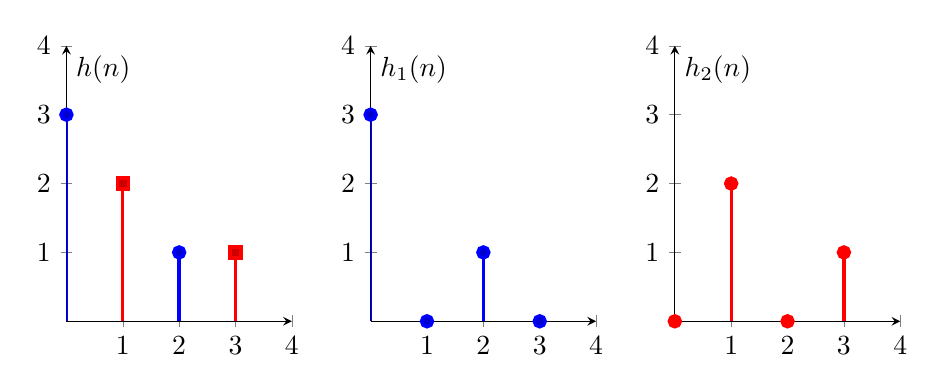
\begin{tikzpicture}
    \begin{groupplot}[
        group style={group size=3 by 1},
        axis lines=middle,
        width=1.75in,
        height=2in,
        ymax=4]
      \nextgroupplot[ylabel=$h(n)$, xmin=0, xmax=4, ymin=0];
      \addplot+[ycomb, line width=1.2pt, color=blue] plot coordinates {(0, 3) (2, 1)};
      \addplot+[ycomb, line width=1.2pt, color=red] plot coordinates {(1, 2) (3, 1)};
      \nextgroupplot[ylabel=$h_1(n)$, xmin=0, xmax=4, ymin=0];
      \addplot+[ycomb, line width=1.2pt] plot coordinates {(0, 3) (1, 0) (2, 1) (3, 0)};
      \nextgroupplot[ylabel=$h_2(n)$, xmin=0, xmax=4, ymin=0];
      \addplot+[ycomb, line width=1.2pt, color=red, mark options={red}] plot coordinates {(0, 0) (1, 2) (2, 0) (3, 1)};
    \end{groupplot}
  \end{tikzpicture}
  \caption{Example: M=2}
\end{figure}

This means if we let $e_k[n] = h_k[nM]$, we can utilize the linearity of convolution to build a bank of filters.
\begin{figure}[H]
  \centering
  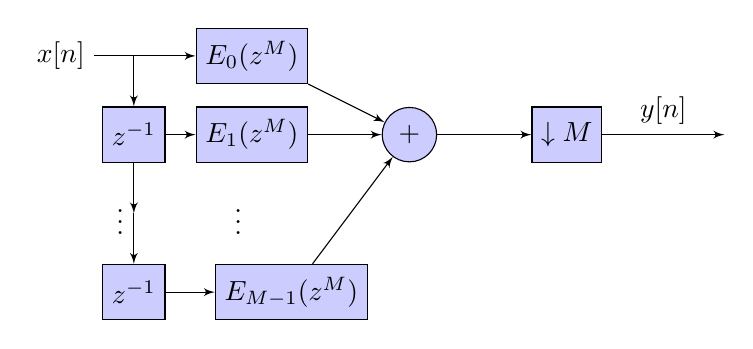
\begin{tikzpicture}[node distance=2cm,auto,>=latex']
      \node (start) [coordinate] {};
      \node (div) [coordinate, right of=start, node distance=0.5cm] {};

      \node [int] (f1) [right of=start, node distance=2cm] {$E_0(z^M)$};
      \node [int] (d1) [below of=div, node distance=1cm] {$z^{-1}$};

      \node [int] (f2) [below of=f1, node distance=1cm] {$E_1(z^M)$};
      \node (de) [coordinate, below of=d1, node distance=1cm] {};
      
      \node (e) [below of=f2, node distance=1cm, coordinate] {};
      \node [int] (dm) [below of=de, node distance=1cm] {$z^{-1}$};

      \node [int] (fm) [right of=dm, node distance=2cm] {$E_{M-1}(z^M)$};

      \node [sum] (add) [right of=f2, node distance=2cm] {+};
      \node [int] (down) [right of=add, node distance=2cm]{$\downarrow M$};
      \node (out) [coordinate, right of=down, node distance=2cm] {};

      \draw[] (start) edge node {$x[n]$} (start);
      \draw[] (de) edge node {$\vdots$} (de);
      \draw[] (e) edge node {$\vdots$} (e);
      \draw[] (out) edge node {} (out);

      \path[->] (start) edge node {} (f1);
      \path[->] (f1) edge node {} (add);
      \path[->] (f2) edge node {} (add);
      \path[->] (fm) edge node {} (add);
      \path[->] (add) edge node {} (down);
      \path[->] (down) edge node {$y[n]$} (out);

      \path[->] (div) edge node {} (d1);
      \path[->] (d1) edge node {} (f2);
      \path[->] (d1) edge node {} (de);
      \path[->] (de) edge node {} (dm);
      \path[->] (dm) edge node {} (fm);
  \end{tikzpicture}    
\end{figure}
Now each of our filters is compressible, so we can switch the order of downsampling and filtering while maintaining the same output.
\begin{figure}[H]
  \centering
  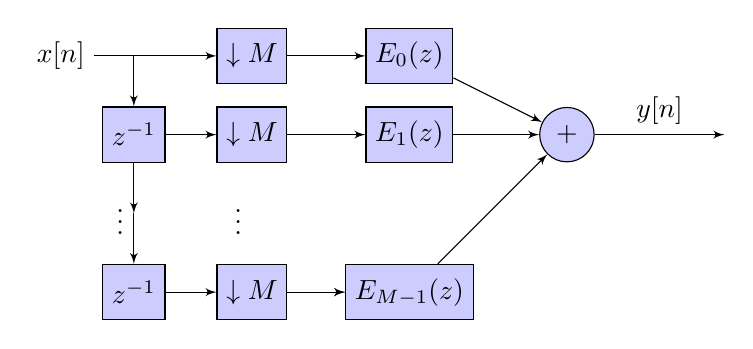
\begin{tikzpicture}[node distance=2cm,auto,>=latex']
      \node (start) [coordinate] {};
      \node (div) [coordinate, right of=start, node distance=0.5cm] {};

      \node [int] (down1) [right of=start, node distance=2cm]{$\downarrow M$};
      \node [int] (f1) [right of=down1, node distance=2cm] {$E_0(z)$};
      \node [int] (d1) [below of=div, node distance=1cm] {$z^{-1}$};

      \node [int] (down2) [below of=down1, node distance=1cm]{$\downarrow M$};
      \node [int] (f2) [below of=f1, node distance=1cm] {$E_1(z)$};
      \node (de) [coordinate, below of=d1, node distance=1cm] {};
      
      \node (e) [below of=down2, node distance=1cm, coordinate] {};
      \node [int] (dm) [below of=de, node distance=1cm] {$z^{-1}$};
      \node [int] (downm) [right of=dm, node distance=1.5cm]{$\downarrow M$};

      \node [int] (fm) [right of=downm, node distance=2cm] {$E_{M-1}(z)$};

      \node [sum] (add) [right of=f2, node distance=2cm] {+};
      \node (out) [coordinate, right of=add, node distance=2cm] {};

      \draw[] (start) edge node {$x[n]$} (start);
      \draw[] (de) edge node {$\vdots$} (de);
      \draw[] (e) edge node {$\vdots$} (e);
      \draw[] (out) edge node {} (out);

      \path[->] (start) edge node {} (down1);
      \path[->] (down1) edge node {} (f1);
      \path[->] (down2) edge node {} (f2);
      \path[->] (downm) edge node {} (fm);
      \path[->] (f1) edge node {} (add);
      \path[->] (f2) edge node {} (add);
      \path[->] (fm) edge node {} (add);
      \path[->] (add) edge node {$y[n]$} (out);

      \path[->] (div) edge node {} (d1);
      \path[->] (d1) edge node {} (down2);
      \path[->] (d1) edge node {} (de);
      \path[->] (de) edge node {} (dm);
      \path[->] (dm) edge node {} (downm);
      \path[->] (downm) edge node {} (fm);
  \end{tikzpicture}    
\end{figure}
Now for any filter, we can compute only what we need, so the result is correct and efficently obtained.
\subsection{Practical Sampling (ADC)}
Unfortunately, ideal analog to digital conversion is not possible for a variety of reasons. The first is that not all signals are bandlimited (or there may be noise outside of the bandwidth).
Moreover, computers only have finite precision, so we cannot represent the full range of values that a continuous signal might take on with a finite number of bits per sample. The solution to the first issue is to include a "anti-aliasing" filter before the sampler. 
The solution to the second issue is to quantize.
\begin{figure}[H]
  \centering
  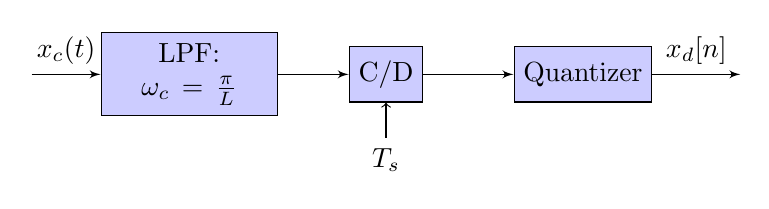
\begin{tikzpicture}[node distance=2.5cm,auto,>=latex']
      \node [filter] (a) {LPF:\\$\omega_c=\frac{\pi}{L}$};
      \node (b) [left of=a,node distance=2cm, coordinate] {x(t)};
      \node [int, pin={[init]below:$T_s$}] (c) [right of=a] {C/D};
      \node [int] (d) [right of=c] {Quantizer};
      \node [coordinate] (end) [right of=d, node distance=2cm]{};
      \path[->] (b) edge node {$x_c(t)$} (a);
      \path[->] (a) edge node {} (c);
      \draw[->] (c) edge node {} (d) ;
      \draw[->] (d) edge node {$x_d[n]$} (end) ;
  \end{tikzpicture}    
\end{figure}
However, sharp analog filters are difficult to implement in practice. To deal with this,
we could make the anti-aliasing filter wider, but this would add noise and interference. If we keep the cutoff frequency the same,
then we could alter part of the signal because our filter is not ideal. A better solution is to do the processing in Discrete Time
because we have more control. We also sample higher than the Nyquist Rate and then downsample it to the required rate.
\begin{figure}[H]
  \centering
  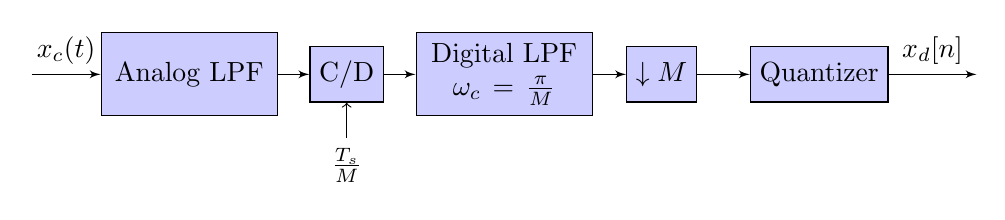
\begin{tikzpicture}[node distance=2.5cm,auto,>=latex']
      \node [filter] (a) {Analog LPF};
      \node (b) [left of=a,node distance=2cm, coordinate] {x(t)};
      \node [int, pin={[init]below:$\frac{T_s}{M}$}, node distance=2cm] (c) [right of=a] {C/D};
      \node [filter, node distance=2cm] (d) [right of=c] {Digital  LPF\\$\omega_c=\frac{\pi}{M}$};
      \node [int] (e) [right of=d, node distance=2cm] {$\downarrow M$};
      \node [int] (f) [right of=e, node distance=2cm] {Quantizer};
      \node [coordinate] (end) [right of=f, node distance=2cm]{};
      \path[->] (b) edge node {$x_c(t)$} (a);
      \path[->] (a) edge node {} (c);
      \draw[->] (c) edge node {} (d) ;
      \draw[->] (d) edge node {} (e) ;
      \draw[->] (e) edge node {} (f) ;
      \draw[->] (f) edge node {$x_d[n]$} (end) ;
  \end{tikzpicture}    
\end{figure}
\subsubsection{Quantization}
If we have a dynamic range of $X_m$ (i.e $2X_m$ is the length of the range of values we can represent), then
our step between quantized values is $\Delta=\frac{X_m}{2^B}$, assuming we are representing our data as 2's complement 
numbers with $B$ bits. We model the error caused by quantization as additive noise. Our quantized signal $\hat{x}[n]$ is decribed by
$$\hat{x}[n] = x[n] + e[n] \qquad \frac{-\Delta}{2}\le e[n] \le \frac{\Delta}{2}$$
We do this under the following assumptions:
\begin{itemize}
  \item $e[n]$ is produced by a stationary random process
  \item $e[n]$ is not correlated with $x[n]$
  \item $e[n]$ is white noise ($e[n]$ is not correlated with $e[m]$)
  \item $e[n]\sim U\left[\frac{-\Delta}{2},\frac{\Delta}{2}\right]$ 
\end{itemize}
For rapidly changing signals with small $\Delta$, this assumptions hold, and they are useful in modeling quantization error.
Since $\Delta = 2^{-B}X_m$
$$\sigma^2_e=\frac{\Delta^2}{12}=\frac{2^{-2B}X_m^2}{12}$$
This means our Signal to Noise Ratio for quantization is
$$SNR_Q=10\log\left(\frac{\sigma_x^2}{\sigma_e^2}\right)=6.02B+10.8-20\log\left(\frac{X_m}{\sigma_s}\right)$$
What this tells us is that every new bit we add gives us 6dB in improvement. It also tells us that we need to
adapt the range of quantization to the RMS amplitude of the signal. This means there is a tradeoff between clipping and quantization noise.
When we oversampling our signal, we can further limit the effects of quantization noise because this noise will be spread out over more frequencies
and the LPF will eliminate noise outside the signal bandwidth. This makes $\frac{\sigma_e^2}{M}$ the new noise variance (if we oversample by $M$).
Thus we can modify the $SNR_Q$ equation
$$SNR_Q=6.02B+10.8-20\log\left(\frac{X_m}{\sigma_s}\right) + 10\log M$$
This shows that doubling $M$ yields a 3dB improvement (equivalent to 0.5 more bits).
\subsection{Practice Reconstruction (DAC)}
In the ideal case, we reconstruct signals by converting them to impulses and then convolving with a sinc.
However, impulses are require lots of power to generate, and sincs are infinitely long, so it is impractical to design an analog system to do this.
Instead, we use an interpolation like Zero-Order-Hold to pulses and then filter with a reconstruction filter.
\begin{figure}[H]
  \centering
  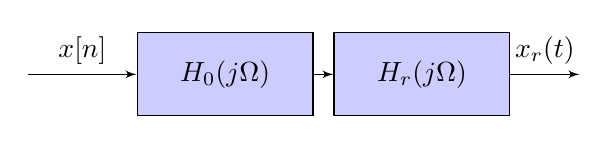
\begin{tikzpicture}[node distance=2.5cm,auto,>=latex']
      \node [filter] (a) {$H_0(j\Omega)$};
      \node (b) [left of=a,coordinate] {x(t)};
      \node [filter] (c) [right of=a] {$H_r(j\Omega)$};
      \node [coordinate] (end) [right of=c, node distance=2cm]{};
      \path[->] (b) edge node {$x[n]$} (a);
      \path[->] (a) edge node {} (c);
      \draw[->] (c) edge node {$x_r(t)$} (end);
  \end{tikzpicture}    
\end{figure}
$$X_r(j\Omega) = H_r(j\Omega)\overbrace{Te^{-j\Omega\frac{T}{2}}sinc\left(\frac{\Omega}{\Omega_s}\right)}^{\text{Zero Order Hold}}\overbrace{\frac{1}{T}\sum_{k=-\infty}^{\infty}X(j(\Omega-k\Omega_s))}^{\text{Sampled Signal}}$$
We design $H_r(j\Omega)$ such that $H_r(j\omega)H_0(j\omega)$ is approximately an LPF.
\end{document}